\section{Công nghệ và quyết định lựa chọn}

Chương này trình bày các công nghệ được sử dụng trong hệ thống và lý do lựa chọn chúng. Nội dung được tổ chức theo luồng xử lý từ giao diện, Backend nghiệp vụ, AI Service, xử lý đa phương thức, truy hồi đến hạ tầng triển khai. Các nguyên lý lý thuyết đã được trình bày ở Chương 2; kiến trúc chi tiết và quy trình cài đặt lần lượt thuộc Chương 7 và Chương 8 nên không lặp lại tại đây.

\subsection{Tiêu chí và tổng quan lựa chọn công nghệ}

Các công nghệ được lựa chọn theo năm tiêu chí chính:

\begin{itemize}
    \item đáp ứng các chức năng thương mại điện tử, tìm kiếm đa phương thức và hội thoại RAG;
    \item phù hợp với dữ liệu, mã nguồn và năng lực triển khai của đề tài;
    \item có hợp đồng giao tiếp rõ ràng, thuận tiện kiểm thử và thay thế thành phần;
    \item vận hành được bằng container trong cả môi trường cục bộ và Google Cloud;
    \item cân bằng chất lượng, độ trễ, chi phí và yêu cầu quản trị hạ tầng.
\end{itemize}

Theo các tiêu chí trên, hệ thống sử dụng React ở lớp giao diện, Spring Boot và MySQL ở lớp nghiệp vụ, FastAPI và LangGraph ở AI Service, Cohere Embed v4 cùng Qdrant cho truy hồi đa phương thức, và Docker--Google Cloud cho triển khai. Redis được dùng cho trạng thái hội thoại ở môi trường Cloud Run. YOLOv26 hỗ trợ phát hiện vùng sản phẩm trong môi trường có cài mô hình cục bộ; cấu hình Cloud Run sử dụng ảnh đầy đủ để tránh phụ thuộc GPU và thư viện thị giác nặng.

\subsection{Công nghệ xây dựng giao diện}

\subsubsection{React}

Frontend sử dụng React 19 để xây dựng giao diện theo component \parencite{reactdocs2024}. Mô hình này phù hợp với các màn hình có nhiều trạng thái tương tác như bộ lọc, danh sách kết quả, thẻ sản phẩm, giỏ hàng, vùng tải ảnh và hội thoại nhiều lượt. Các component có thể tái sử dụng giữa tìm kiếm văn bản, hình ảnh và kết hợp mà không phải nhân bản toàn bộ giao diện.

React được chọn thay vì một framework full-stack vì Frontend của hệ thống chỉ giao tiếp với Spring Boot qua REST API, không đảm nhiệm nghiệp vụ hoặc truy cập trực tiếp dữ liệu. Hạn chế chính là trạng thái có thể trở nên phức tạp khi nhiều request cập nhật đồng thời; do đó trạng thái tìm kiếm, hội thoại và nghiệp vụ được tách theo từng nhóm chức năng.

\subsubsection{Redux Toolkit, React Router và Axios}

Redux Toolkit quản lý các trạng thái dùng chung như phiên đăng nhập, giỏ hàng và dữ liệu cần chia sẻ giữa nhiều màn hình. React Router tổ chức điều hướng phía client; Axios đảm nhiệm lời gọi HTTP và cho phép xử lý tập trung token, timeout cùng lỗi API. Bootstrap và SCSS cung cấp hệ thống bố cục responsive, còn Vite đảm nhiệm dev server và quá trình build.

Nhóm thư viện này được lựa chọn vì phù hợp với ứng dụng React dạng single-page application và giảm lượng mã nền phải tự xây dựng. Các thư viện chỉ xử lý trình bày và giao tiếp; mọi quyết định về quyền truy cập, giá, tồn kho và trạng thái đơn hàng vẫn do Backend xác nhận.

\subsection{Công nghệ Backend và dữ liệu nghiệp vụ}

\subsubsection{Java và Spring Boot}

Backend sử dụng Java 21 và Spring Boot 4.0.6. Spring Boot cung cấp auto-configuration, embedded server và hệ sinh thái xây dựng REST API \parencite{springbootdocs2024}. Công nghệ này phù hợp với nghiệp vụ thương mại điện tử có nhiều ràng buộc giao dịch như giỏ hàng, tồn kho, khuyến mãi, đơn hàng và thanh toán COD.

Spring Boot được chọn vì hỗ trợ transaction, validation, security và truy cập dữ liệu quan hệ đồng bộ trong một nền tảng thống nhất. So với một API Python tối giản, ứng dụng Java có thời gian khởi động và cấu hình lớn hơn; vì vậy phần suy luận AI được tách sang FastAPI thay vì đưa vào cùng tiến trình Backend.

\subsubsection{Spring Security, JPA và RestClient}

Spring Web MVC được dùng cho controller và REST endpoint; Spring Data JPA ánh xạ entity và truy cập MySQL; Spring Security cùng OAuth2 Client xử lý xác thực và phân quyền. RestClient thực hiện giao tiếp nội bộ với AI Service, còn Spring AOP và AspectJ hỗ trợ các tác vụ cắt ngang như ghi log hoặc kích hoạt đồng bộ catalog.

Việc sử dụng các module trong cùng hệ sinh thái giúp chính sách transaction, validation và lỗi API nhất quán. Backend đồng thời là cổng giao tiếp duy nhất của Frontend, nhờ đó khóa dịch vụ AI, Qdrant và cơ sở dữ liệu không bị đưa ra phía trình duyệt.

\subsubsection{MySQL}

MySQL 8.4 lưu dữ liệu nghiệp vụ gồm tài khoản, phân quyền, danh mục, sản phẩm, biến thể, giá, tồn kho, giỏ hàng, khuyến mãi và đơn hàng. MySQL được chọn vì mô hình quan hệ phù hợp với các ràng buộc khóa ngoại và giao dịch cần thiết cho thương mại điện tử, đồng thời được hỗ trợ trực tiếp bởi Spring Data JPA.

Trong hệ thống, MySQL là nguồn dữ liệu chuẩn. Qdrant chỉ đóng vai trò chỉ mục có thể tái tạo; kết quả AI chỉ chứa mã sản phẩm và điểm số, sau đó Backend đọc lại giá, tồn kho cùng trạng thái hiện hành từ MySQL trước khi trả cho người dùng.

\subsection{Công nghệ xây dựng AI Service}

\subsubsection{Python, FastAPI và Pydantic}

AI Service sử dụng Python 3.11 và FastAPI. FastAPI hỗ trợ API theo chuẩn ASGI, xử lý bất đồng bộ và sinh OpenAPI từ type hints \parencite{fastapidocs2024}. Pydantic xác thực, chuẩn hóa request/response; HTTPX thực hiện lời gọi tới Spring Boot và các dịch vụ mô hình; Pillow giải mã, resize và crop ảnh.

FastAPI được chọn vì hệ sinh thái Python thuận lợi cho embedding, xử lý ảnh và điều phối mô hình. Ranh giới REST giúp thay đổi provider embedding, LLM hoặc reranker mà không làm thay đổi giao diện người dùng. Đổi lại, hợp đồng giữa Backend và AI Service phải được kiểm soát phiên bản, timeout và lỗi fallback rõ ràng.

\subsubsection{LangGraph và Redis}

LangGraph điều phối workflow hội thoại có trạng thái dưới dạng graph \parencite{langgraph2024docs}. Các node thực hiện tải ngữ cảnh, hiểu truy vấn, định tuyến, truy hồi, lấy dữ liệu sản phẩm và sinh phản hồi; conditional edge quyết định nhánh xử lý theo ý định cùng dữ liệu đầu vào. LangGraph phù hợp hơn một chain tuyến tính vì trợ lý cần clarification, memory recall và nhiều đường đi có kiểm soát.

Ở môi trường Cloud Run, Redis lưu checkpoint và preference memory có thời hạn. Redis hỗ trợ truy cập nhanh và chia sẻ trạng thái ngoài tiến trình, phù hợp khi container AI Service có thể được thay thế. SQLite chỉ dùng cho phát triển hoặc kiểm thử đơn instance. Hệ thống không xem workflow này là agent tự trị: các node, công cụ và điều kiện chuyển trạng thái đều được giới hạn trước.

\subsubsection{LLM qua Amazon Bedrock}

Cấu hình triển khai sử dụng mô hình ngôn ngữ được quản lý qua Amazon Bedrock. LLM đảm nhiệm phân tích ý định, trích xuất thuộc tính, viết lại truy vấn và diễn đạt câu trả lời; dữ kiện về sản phẩm được cung cấp bởi tầng truy hồi và Backend thay vì lấy từ tri thức tham số của mô hình.

Dịch vụ managed giúp không phải vận hành GPU cho LLM và cho phép thay model qua cấu hình. Hạn chế là phụ thuộc vào mạng, quota, chi phí và chính sách provider; vì vậy AI Service áp dụng timeout, retry có giới hạn, fallback và ghi nhận model cùng độ trễ cho từng lần gọi.

\subsection{Công nghệ xử lý ảnh và embedding đa phương thức}

\subsubsection{YOLOv26 và Pillow}

YOLO được lựa chọn cho bước phát hiện vùng chứa sản phẩm nhờ kiến trúc one-stage và khả năng suy luận nhanh \parencite{redmon2016yolo}. Trong đồ án, YOLOv26s được fine-tune trên dữ liệu thời trang để nhận diện bốn nhóm tổng quát gồm phụ kiện, túi, quần áo và giày. Bounding box có độ tin cậy phù hợp được dùng để crop sản phẩm trước khi tạo image embedding; Pillow thực hiện các thao tác giải mã và chuẩn hóa ảnh.

YOLO là bước tăng cường, không phải điều kiện bắt buộc của Image Search. Khi không phát hiện được vùng đủ tin cậy, hệ thống sử dụng ảnh đầy đủ. Mô hình được sử dụng trong môi trường cục bộ có cài Ultralytics; image Cloud Run dạng managed-only tắt YOLO và luôn dùng ảnh đầy đủ để giảm kích thước container cùng yêu cầu tài nguyên.

\subsubsection{Cohere Embed v4 qua Amazon Bedrock}

Cấu hình được đánh giá sử dụng \texttt{cohere.embed-v4:0} qua Amazon Bedrock để tạo vector 1.536 chiều cho cả văn bản và hình ảnh. Nhánh văn bản biểu diễn truy vấn và mô tả sản phẩm; nhánh hình ảnh biểu diễn ảnh catalog và ảnh do người dùng cung cấp. Hai loại vector được lưu ở hai collection riêng để tránh trộn modality và thuận tiện đánh giá độc lập.

Multimodal embedding managed giúp thống nhất không gian biểu diễn mà không phải phục vụ các mô hình vision--language cục bộ. Đổi lại, hệ thống chịu độ trễ mạng, quota và chi phí theo request. PyTorch, Transformers, Sentence-Transformers và OpenCLIP chỉ thuộc cấu hình \texttt{local-models} tùy chọn, không phải pipeline production được dùng trong đánh giá cuối.

\subsection{Công nghệ truy hồi và xếp hạng}

\subsubsection{Qdrant}

Qdrant lưu text/image embedding, mã sản phẩm và metadata phục vụ lọc \parencite{qdrant_docs}. Hệ thống duy trì collection riêng cho từng modality; mỗi point liên kết với \texttt{product\_id} và có thể mang các thuộc tính như danh mục, màu, chất liệu, giới tính, giá hoặc trạng thái hoạt động.

\begin{figure}[H]
    \centering
    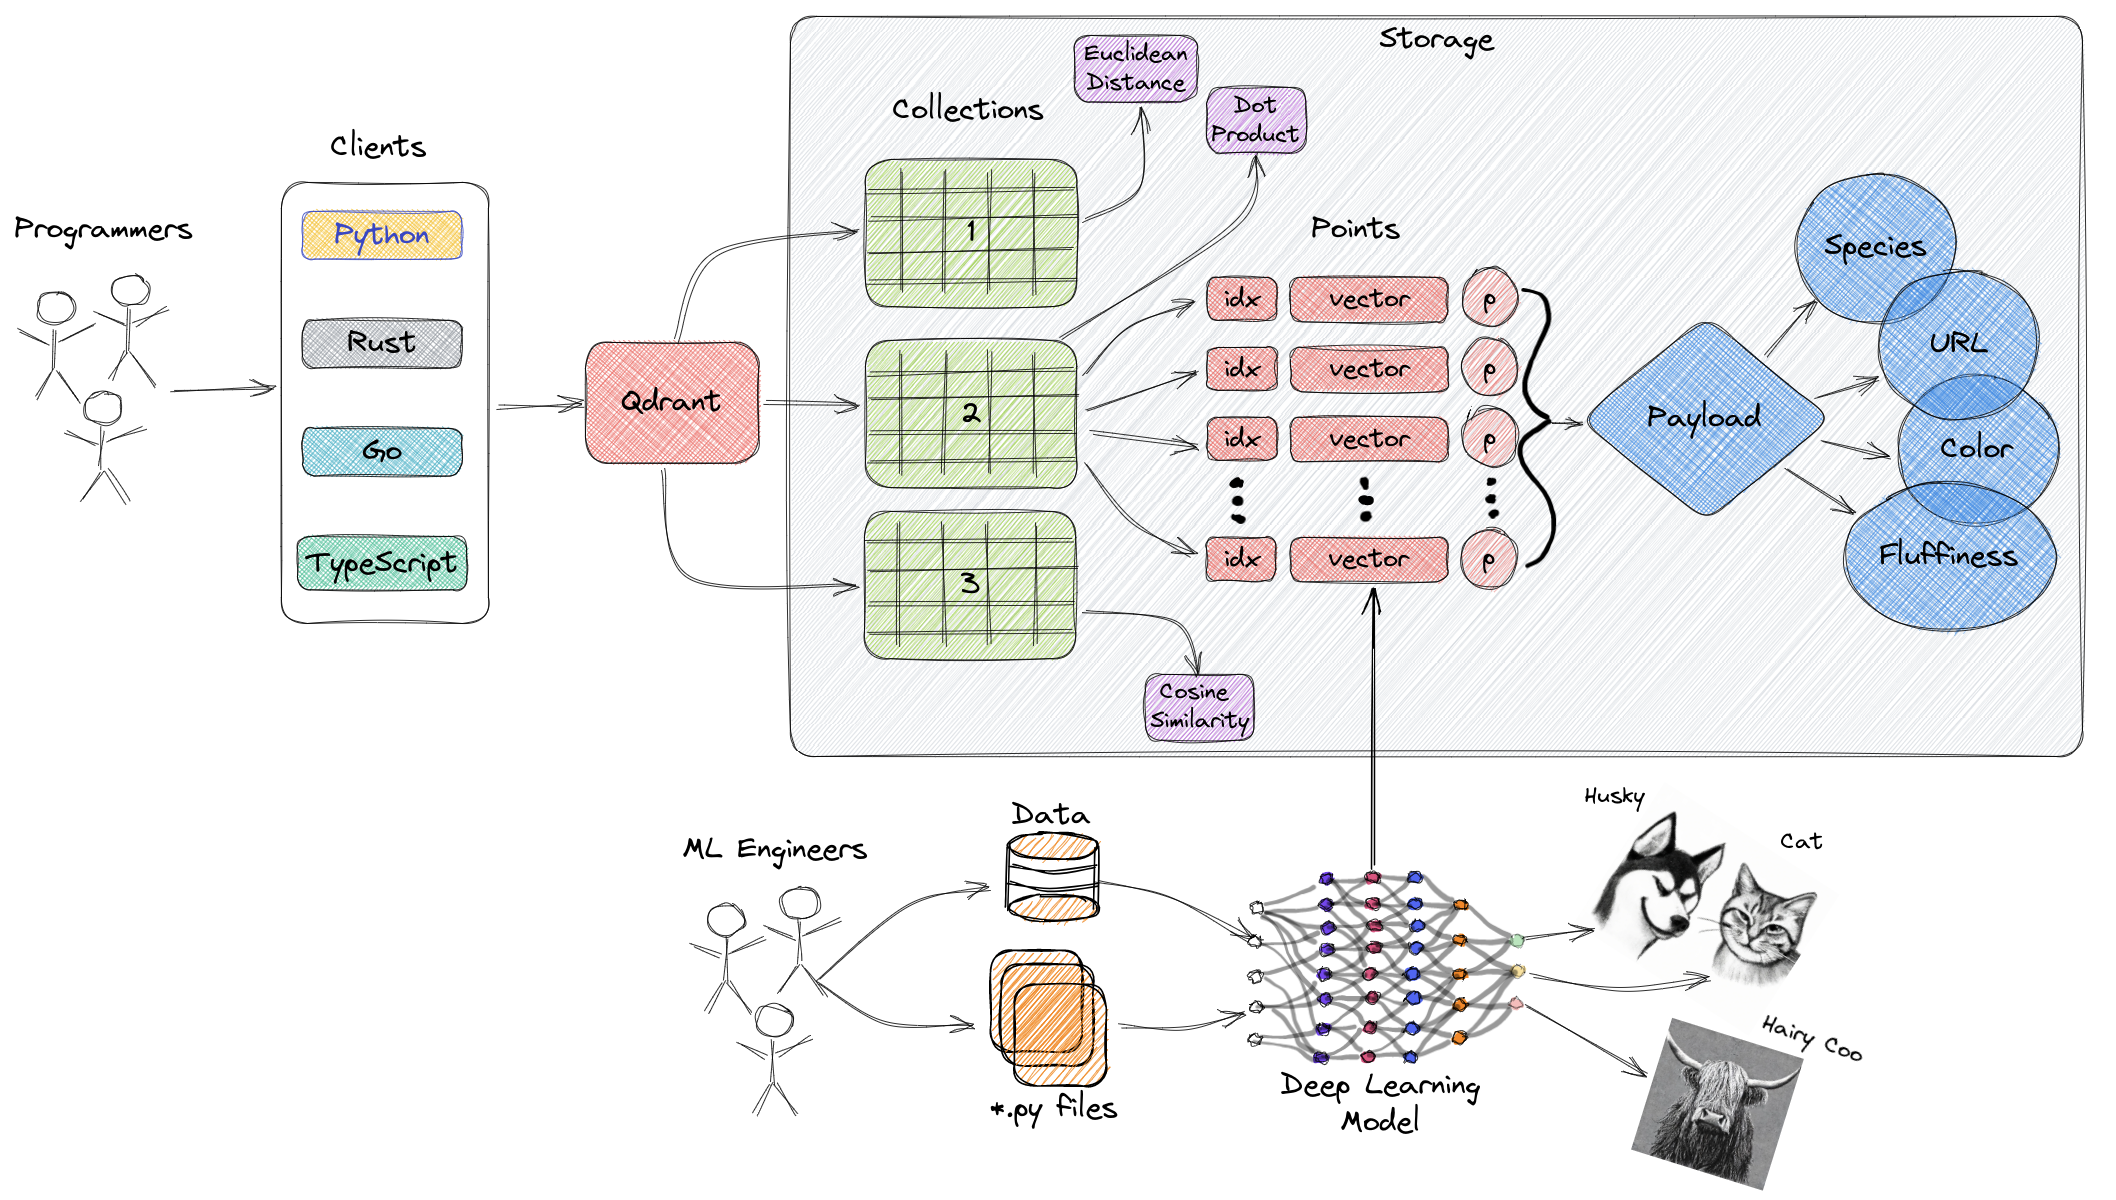
\includegraphics[width=0.86\linewidth]{Images/Congnghelienquan/qdrant_overview_high_level.png}
    \caption{Qdrant kết hợp vector engine, payload và filtering cho truy hồi sản phẩm \parencite{qdrant_overview}}
    \label{fig:selected_qdrant_architecture}
\end{figure}

Qdrant được chọn vì có thể self-host bằng Docker, hỗ trợ độ tương đồng cosine, truy hồi gần đúng bằng HNSW, lọc payload và API Python. So với dịch vụ vector được quản lý hoàn toàn, Qdrant cho phép kiểm soát dữ liệu và chi phí ở quy mô catalog hiện tại; hạn chế là nhóm phát triển phải tự quản lý volume, snapshot, backup và giám sát collection.

\subsubsection{Hybrid fusion và reranker}

Search Service truy hồi ứng viên độc lập từ nhánh văn bản và hình ảnh, quy về \texttt{product\_id}, sau đó hợp nhất điểm với metadata cùng ràng buộc nghiệp vụ. Cách tách first-stage retrieval và fusion giúp điều chỉnh trọng số giữa mức tương đồng ảnh với mức phù hợp văn bản mà không thay đổi vector database.

Google Cloud Ranking API được tích hợp như một reranker managed và chỉ hoạt động khi feature flag được bật. Đây là thành phần xếp hạng tùy chọn, không phải điều kiện của pipeline. Kết quả đánh giá ở Chương 9 cho thấy rerank hiện tại không cải thiện các chỉ số chính, vì vậy cấu hình được lựa chọn để báo cáo là fusion không rerank; API vẫn được giữ để tiếp tục thử nghiệm với mô hình hoặc dữ liệu khác.

\subsection{Công nghệ triển khai}

\subsubsection{Docker và Docker Compose}

Docker đóng gói Frontend, Spring Boot Backend, AI Service, MySQL và Qdrant thành các image hoặc container có cấu hình xác định. Docker Compose mô tả quan hệ phụ thuộc, network, health check và named volume, giúp môi trường phát triển cùng kiểm thử có thể được khởi tạo nhất quán. Frontend và Backend sử dụng build nhiều giai đoạn; Frontend sau khi build được phục vụ bằng nginx.

Container hóa giảm khác biệt môi trường nhưng không thay thế quản trị dữ liệu. MySQL và Qdrant sử dụng volume lâu dài, cần sao lưu trước khi cập nhật; secret và cấu hình môi trường không được đóng trực tiếp vào image.

\subsubsection{Google Compute Engine và Cloud Run}

Bản triển khai Google Cloud sử dụng GCE VM cho Frontend, Spring Boot Backend, MySQL và Qdrant; AI Service được triển khai riêng trên Cloud Run. Cloud Run kết nối tới Backend và Qdrant qua VPC Connector, còn Secret Manager cung cấp Bedrock token, internal API key và Redis URL. Cách phân chia này cho phép cập nhật AI Service độc lập nhưng vẫn giữ cơ sở dữ liệu và vector storage trên volume của VM.

GCE phù hợp với các thành phần cần volume và cấu hình mạng ổn định; Cloud Run phù hợp với AI Service dạng stateless khi checkpoint được đưa sang Redis. Hạn chế của mô hình này là vận hành trải trên hai nền tảng, phát sinh yêu cầu về IAM, private networking, quota, logging và kiểm soát chi phí.

\subsection{Tổng hợp quyết định lựa chọn}

\begin{table}[H]
    \centering
    \caption{Các quyết định công nghệ chính trong phạm vi đồ án}
    \label{tab:technology_decisions}
    \renewcommand{\arraystretch}{1.2}
    \begin{tabularx}{\linewidth}{|p{0.20\linewidth}|X|X|}
        \hline
        \textbf{Thành phần} & \textbf{Lý do lựa chọn} & \textbf{Hạn chế và cách kiểm soát} \\ \hline
        React & Component hóa, phù hợp giao diện tìm kiếm và hội thoại & Tách state theo feature; Backend vẫn xác nhận mọi dữ liệu nghiệp vụ \\ \hline
        Spring Boot--MySQL & Transaction, security và dữ liệu quan hệ phù hợp thương mại điện tử & Tách suy luận AI sang FastAPI; MySQL giữ vai trò nguồn chuẩn \\ \hline
        FastAPI--LangGraph & API Python thuận lợi cho AI và workflow có trạng thái & Kiểm soát graph, timeout, hợp đồng API và fallback \\ \hline
        Bedrock--Cohere & Không cần phục vụ LLM và embedding bằng GPU cục bộ & Theo dõi quota, chi phí, model, độ trễ và lỗi provider \\ \hline
        YOLOv26 & Crop vùng sản phẩm để giảm nhiễu ảnh trong môi trường hỗ trợ & Là bước tùy chọn; dùng ảnh đầy đủ khi tắt hoặc phát hiện thất bại \\ \hline
        Qdrant & Self-host, ANN/HNSW và payload filtering & Quản lý volume, snapshot và khả năng tái lập chỉ mục \\ \hline
        Redis & Chia sẻ checkpoint và memory có TTL ngoài container & Bảo vệ secret, giới hạn dung lượng và chính sách hết hạn \\ \hline
        Docker--GCE--Cloud Run & Tái lập môi trường và tách triển khai AI Service & Chuẩn hóa IAM, network, backup, logging và runbook vận hành \\ \hline
    \end{tabularx}
\end{table}

\subsection*{Kết chương}

Chương này đã trình bày các công nghệ theo đúng vai trò trong luồng hệ thống. React đảm nhiệm giao diện; Spring Boot và MySQL xử lý nghiệp vụ; FastAPI, LangGraph và Redis phục vụ AI Service cùng trạng thái hội thoại; YOLOv26 và Cohere Embed v4 xử lý dữ liệu đa phương thức; Qdrant, fusion và reranker tạo tầng truy hồi--xếp hạng; Docker, GCE và Cloud Run cung cấp môi trường triển khai.

Các lựa chọn thay thế như Pinecone, Milvus, LangChain, LlamaIndex hoặc mô hình embedding cục bộ chỉ có vai trò đối chiếu hay thử nghiệm. Quyết định cuối cùng ưu tiên khả năng tích hợp với hệ thống hiện có, khả năng tái lập và kết quả đánh giá thực nghiệm; chi tiết kiến trúc và cấu hình vận hành được trình bày ở các chương sau.
